\section{Controller in frequency domain}

% Framework
\subsection{Framework}
For this part of the work, we have decided to simplify our system and use 2 states instead of 4. The position and speed of the damper are therefore hidden in the force of the actuator, which is still the controllable input of our system.
\begin{figure}[H]
    \centering
    \includegraphics[width=0.7\textwidth]{resources/png/simplified-system.png}
    \caption{Simplified system of an active mass damper}
    \label{fig:simplified-system}
\end{figure}
The law that governs that system is the following : 
$$
m_{tot}\ddot{x} + c\dot{x} + kx = F_{wind} + F_{damper}
$$
where
\begin{itemize}
    \item $F_{damper} = m_{damper}a_{damper}$
    \item $m_{tot} = m_{building} + m_{damper}$
    \item $x$ is the position of the building relative to its rest position ($x = 0$)
\end{itemize}
Let's now define the input, output and states : 
\begin{itemize}
    \item $u_1 = F_{wind}$
    \item $u_2 = F_{damper}$
    \item $x_1 = x$
    \item $x_2 = \dot{x}$
    \item $y = x_1$ 
\end{itemize}
By doing so, our ABCD matrices are the following :
$$
A = \begin{pmatrix}
    0 & 1\\
    \dfrac{-k}{m_{tot}} & \dfrac{-c}{m_{tot}}\\
\end{pmatrix}
\quad
B = \begin{pmatrix}
    0 & 0\\
    \dfrac{1}{m_{tot}} & \dfrac{1}{m_{tot}}\\
\end{pmatrix}
$$
$$
C = \begin{pmatrix}
    1 & 0\\
\end{pmatrix}
\quad
D = \begin{pmatrix}
    0 & 0\\
\end{pmatrix}
$$

\subsubsection{Constraints and simulation specifications}
We have the following constraints : 
\begin{itemize}
    \item Acceleration of the mass damper between \num{0.3} and \num{0.6}$g$, as advised by Prof. Denoël.
    \item Power injected in the mass of below \SI{10}{\kilo\watt} so as to not have too much electrical consumption.
    \item Lateral movement of the top of the building not above \SI{1}{\meter}.
\end{itemize}
The two scenario we look at are the following : a turbulent wind of maximum \SI{810}{\kilo\newton}, that we represented as a sine function and a constant wind of the same intensity.\par
Here are the values of the different parameters we have chosen : 
\begin{table}[H]
    \centering
    \begin{tabular}{|l|c|c|}
        \hline
        {\bf Mass} & $m_{building} = \SI{1e7}{\kilogram}$ & $m_{damper} = \SI{3e3}{\kilogram}$\\ \hline
        {\bf Spring} & \multicolumn{2}{c|}{$k\approx\SI{4e8}{\newton\per\meter}$}\\ \hline
        {\bf Damper} & \multicolumn{2}{c|}{$c\approx\SI{1.3e6}{\newton\second\per\meter}$}\\ \hline
        {\bf Wind} & \multicolumn{2}{c|}{$F_{max} = \SI{810}{\kilo\newton}$}\\ \hline
    \end{tabular}
    \caption{Numerical values of the system}
    \label{tab:numerical-values}
\end{table}

\subsubsection{Choice of cross-over frequency}
The frequency of our building is of about \SI{1}{\hertz}, as advised by Pr. Denoël, and the frequency of the sinusoidal wind we have decided to study is also of \SI{1}{\hertz}, so we have decided to use a cross-over frequency of \SI{5}{\hertz}. All frequencies above that, probably coming from noise and unwanted phenomena, will be attenuated, while the amplitudes of the frequencies below that, which correspond to the internals of our system, will be amplified.
$$
w_{co} = 2\pi f_{co} \approx \SI{30}{\radian\per\second}
$$

% Transfer function of the open-loop system
\subsection{Transfer function of the open-loop system}
The Bode plots of our open-loop system are given at figure \ref{fig:bode-ol}.
\begin{figure}[H]
    \centering
    \includegraphics[width=0.8\textwidth]{resources/png/bode-ol.png}
    \caption{Bode plots for 2D system.}
    \label{fig:bode-ol}
\end{figure}
As can be seen, every frequency is well attenuated, the high ones as well as the low ones.\par
At the cross-over frequency, the gain of the system is of about \SI{-215}{\deci\bel}. This is not what we want. We would like low frequencies to have a positive gain, high frequencies to have a negative one and the gain at the crossover frequency to be of \SI{0}{\deci\bel}.\par
Furthermore, we need a big enough phase margin at the crossover frequency to be resistant to the delays we will have in our system. In order to do that, we have decided to use a lead compensator as well as a gain. We will not need a low-pass filter as high frequencies will be well attenuated without it.

% Loop shaping
\subsection{Loop shaping}
\subsubsection{Lead compensator}
Let's first start with the desired phase margin. Delays are discussed after, but we want to be able to respond at least to \SI{0.02}{\second} delays, which correspond to the \SI{50}{\hertz} of the actuator's piston \cite{iopscience_delay}.\par
We have decided to have a phase margin of \SI{70}{\degree}. In order to increase the phase margin at the crossover frequency, we have decided to use a lead compensator.\par
Its transfer function is given by : 
$$
G(s) = \dfrac{\frac{s}{w_z} + 1}{\frac{s}{w_p} +1}
$$
We now have to determine the values of the parameters $G_{LC}$, $w_z$ and $w_p$. For a given crossover frequency $\omega_{co}$ and a phase margin $\phi_m$, we can determine the two $w$ in the following way : 
$$
\left\{\begin{array}{l}
    {w_{z}=\tan (\alpha) w_{\mathrm{co}}} \\
    {w_{p}=\frac{w_{\mathrm{co}}}{\tan (\alpha)}}
\end{array}\right.
$$
with $\alpha = \frac{\pi}{4} - \frac{\phi_m}{2}$.\par
For our crossover frequency and our desired value of $\phi_m$, we get that : 
$$
w_z = \num{5.2898} \qquad w_p = \num{170.1385}
$$

\subsubsection{Gain}
After that, we need to add a gain to our system in order to increase the amplitude gains for all frequencies and make it so that the amplitude is at \SI{0}{\deci\bel} at the crossover frequency. That is done by using a constant gain of \num{1.5178e9}. This does not affect the phase but increases the amplitudes of about \SI{183.6}{\deci\bel}, which positions our Bode plot to where we wanted it to be.

\subsubsection{Trade-offs}
The Bode and Nyquist plots of the controlled system are given at figures \ref{fig:bode-control} and \ref{fig:nyquist-control}. As can be seen, the desired results are obtained, and we have a phase margin of \SI{70}{\degree} on the Nyquist plot.
\begin{figure}[H]
    \centering
    \includegraphics[width=0.8\textwidth]{resources/png/bode-control.png}
    \caption{Bode plots of the controlled system}
    \label{fig:bode-control}
\end{figure}
\begin{figure}[H]
    \centering
    \includegraphics[width=0.8\textwidth]{resources/png/nyquist-control.png}
    \caption{Nyquist plot of the controlled system}
    \label{fig:nyquist-control}
\end{figure}
Concerning the impacts on the output signal and control input signal, they are in an acceptable range of values with the parameters we have chosen, as can be seen in figures \ref{fig:controllable-input} and \ref{fig:output}.
\begin{figure}[H]
    \centering
    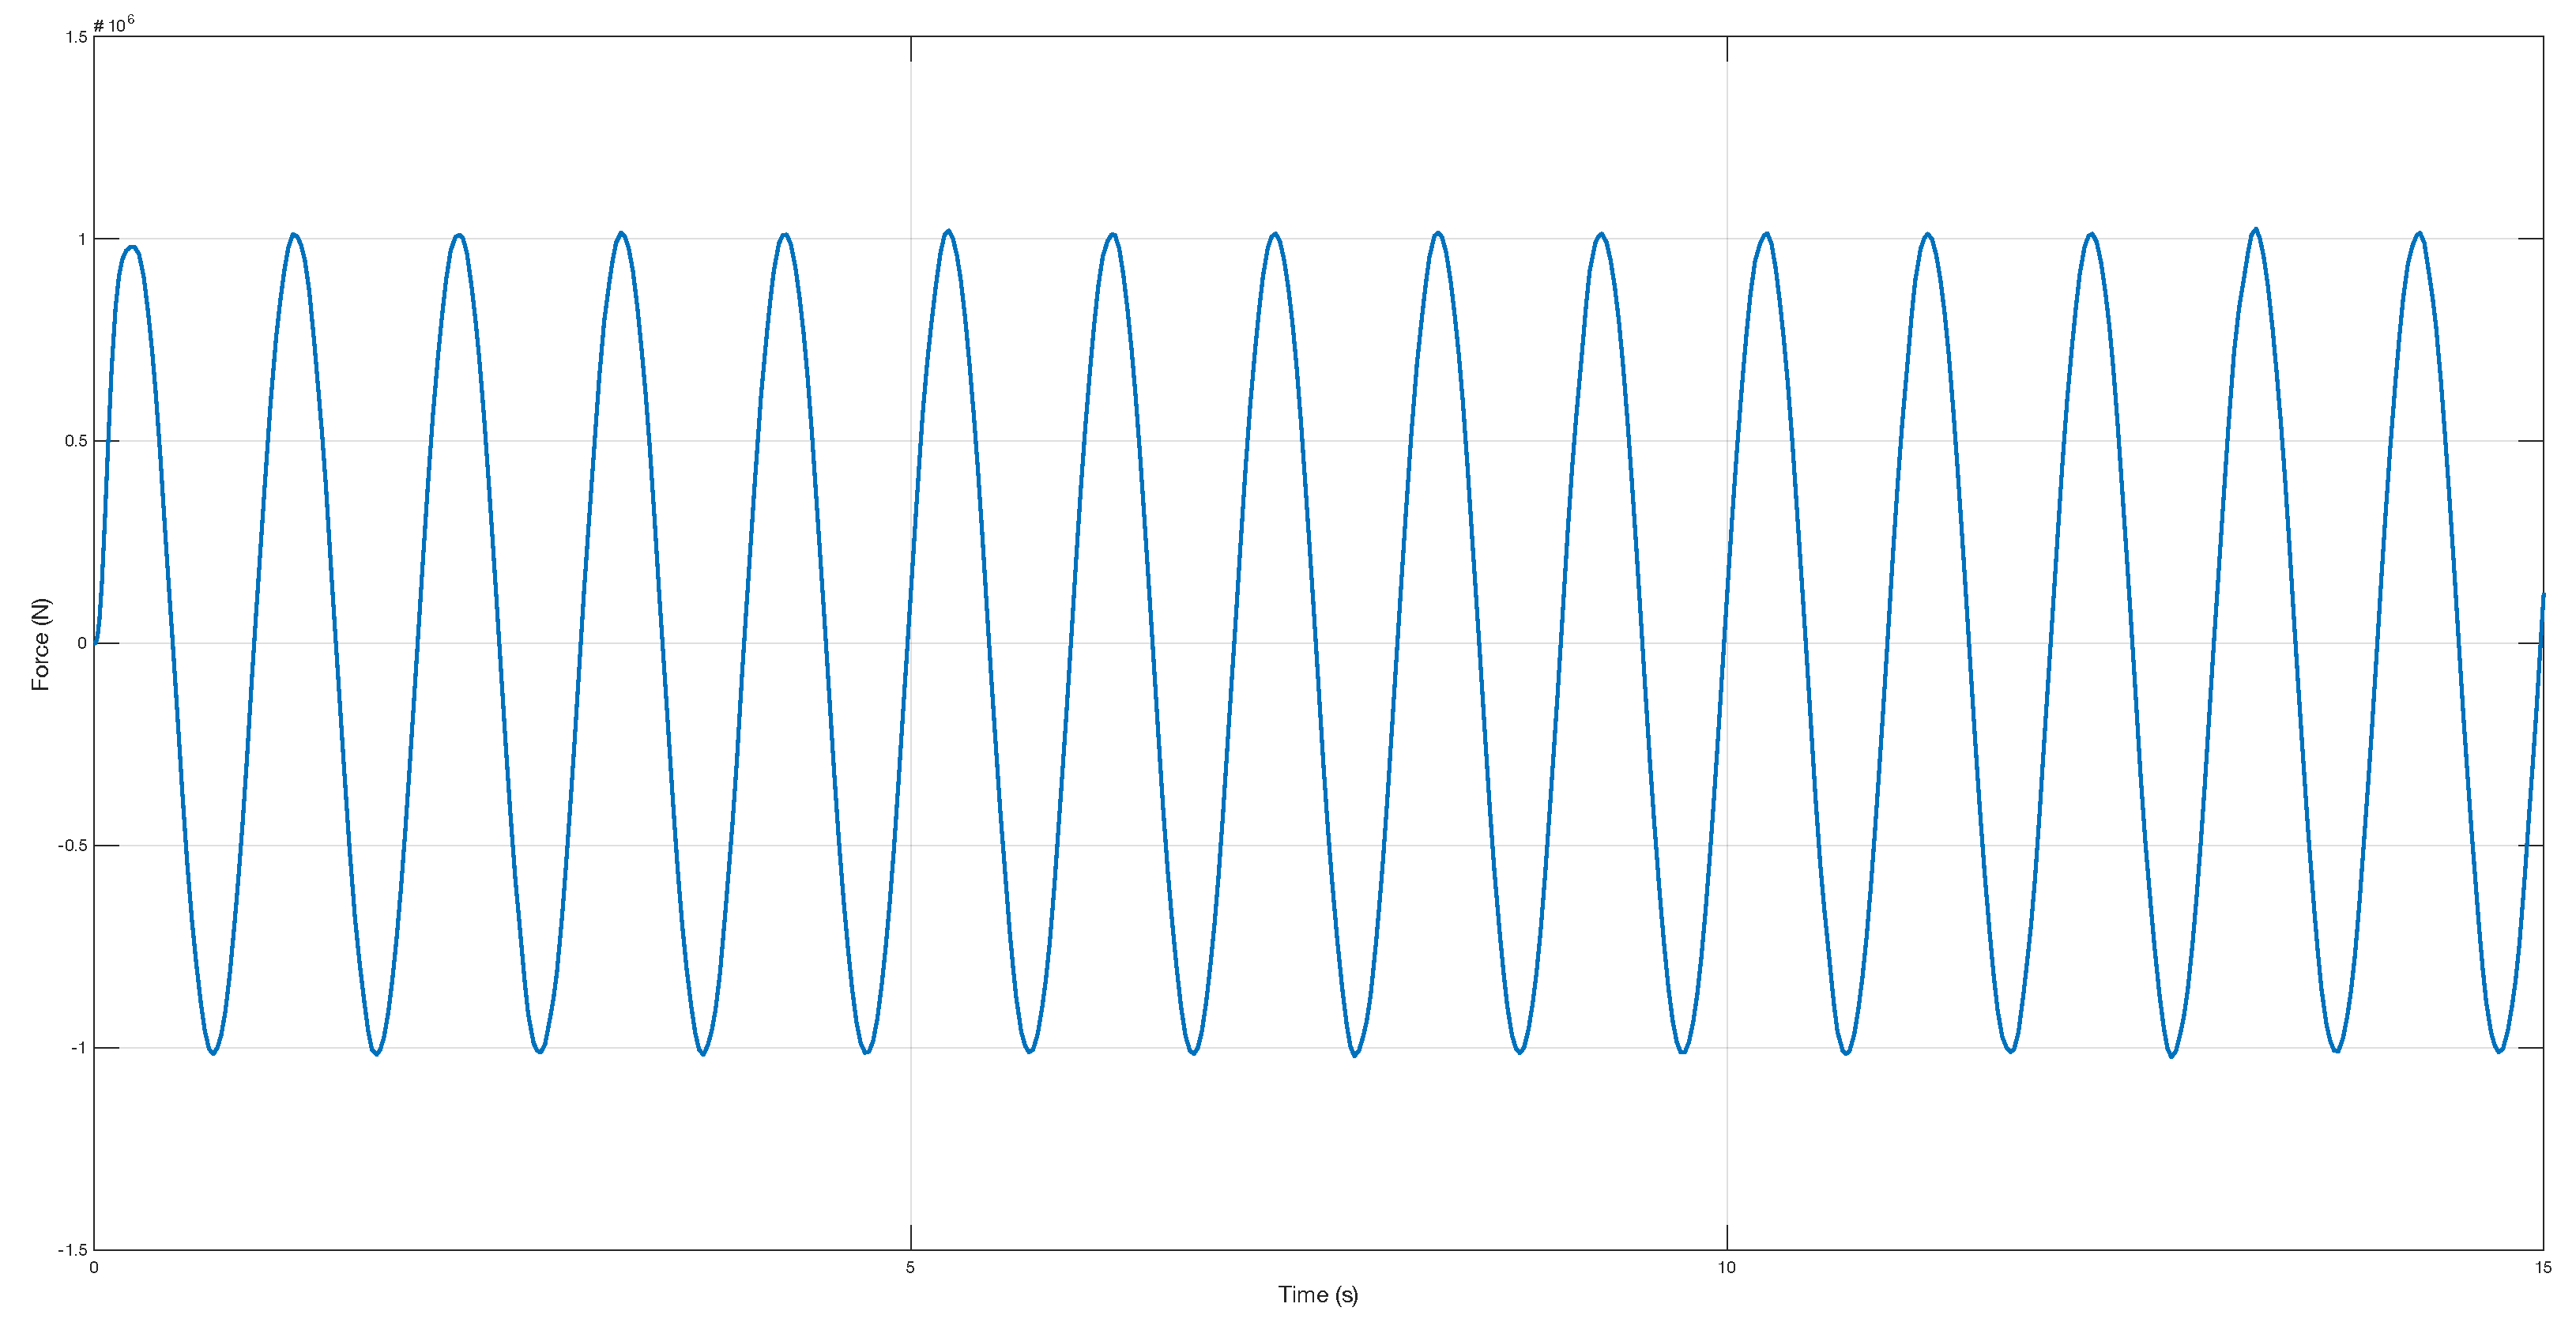
\includegraphics[width=0.8\textwidth]{resources/pdf/controllable-input.pdf}
    \caption{Plot of the controllable input of the controlled system}
    \label{fig:controllable-input}
\end{figure}
\begin{figure}[H]
    \centering
    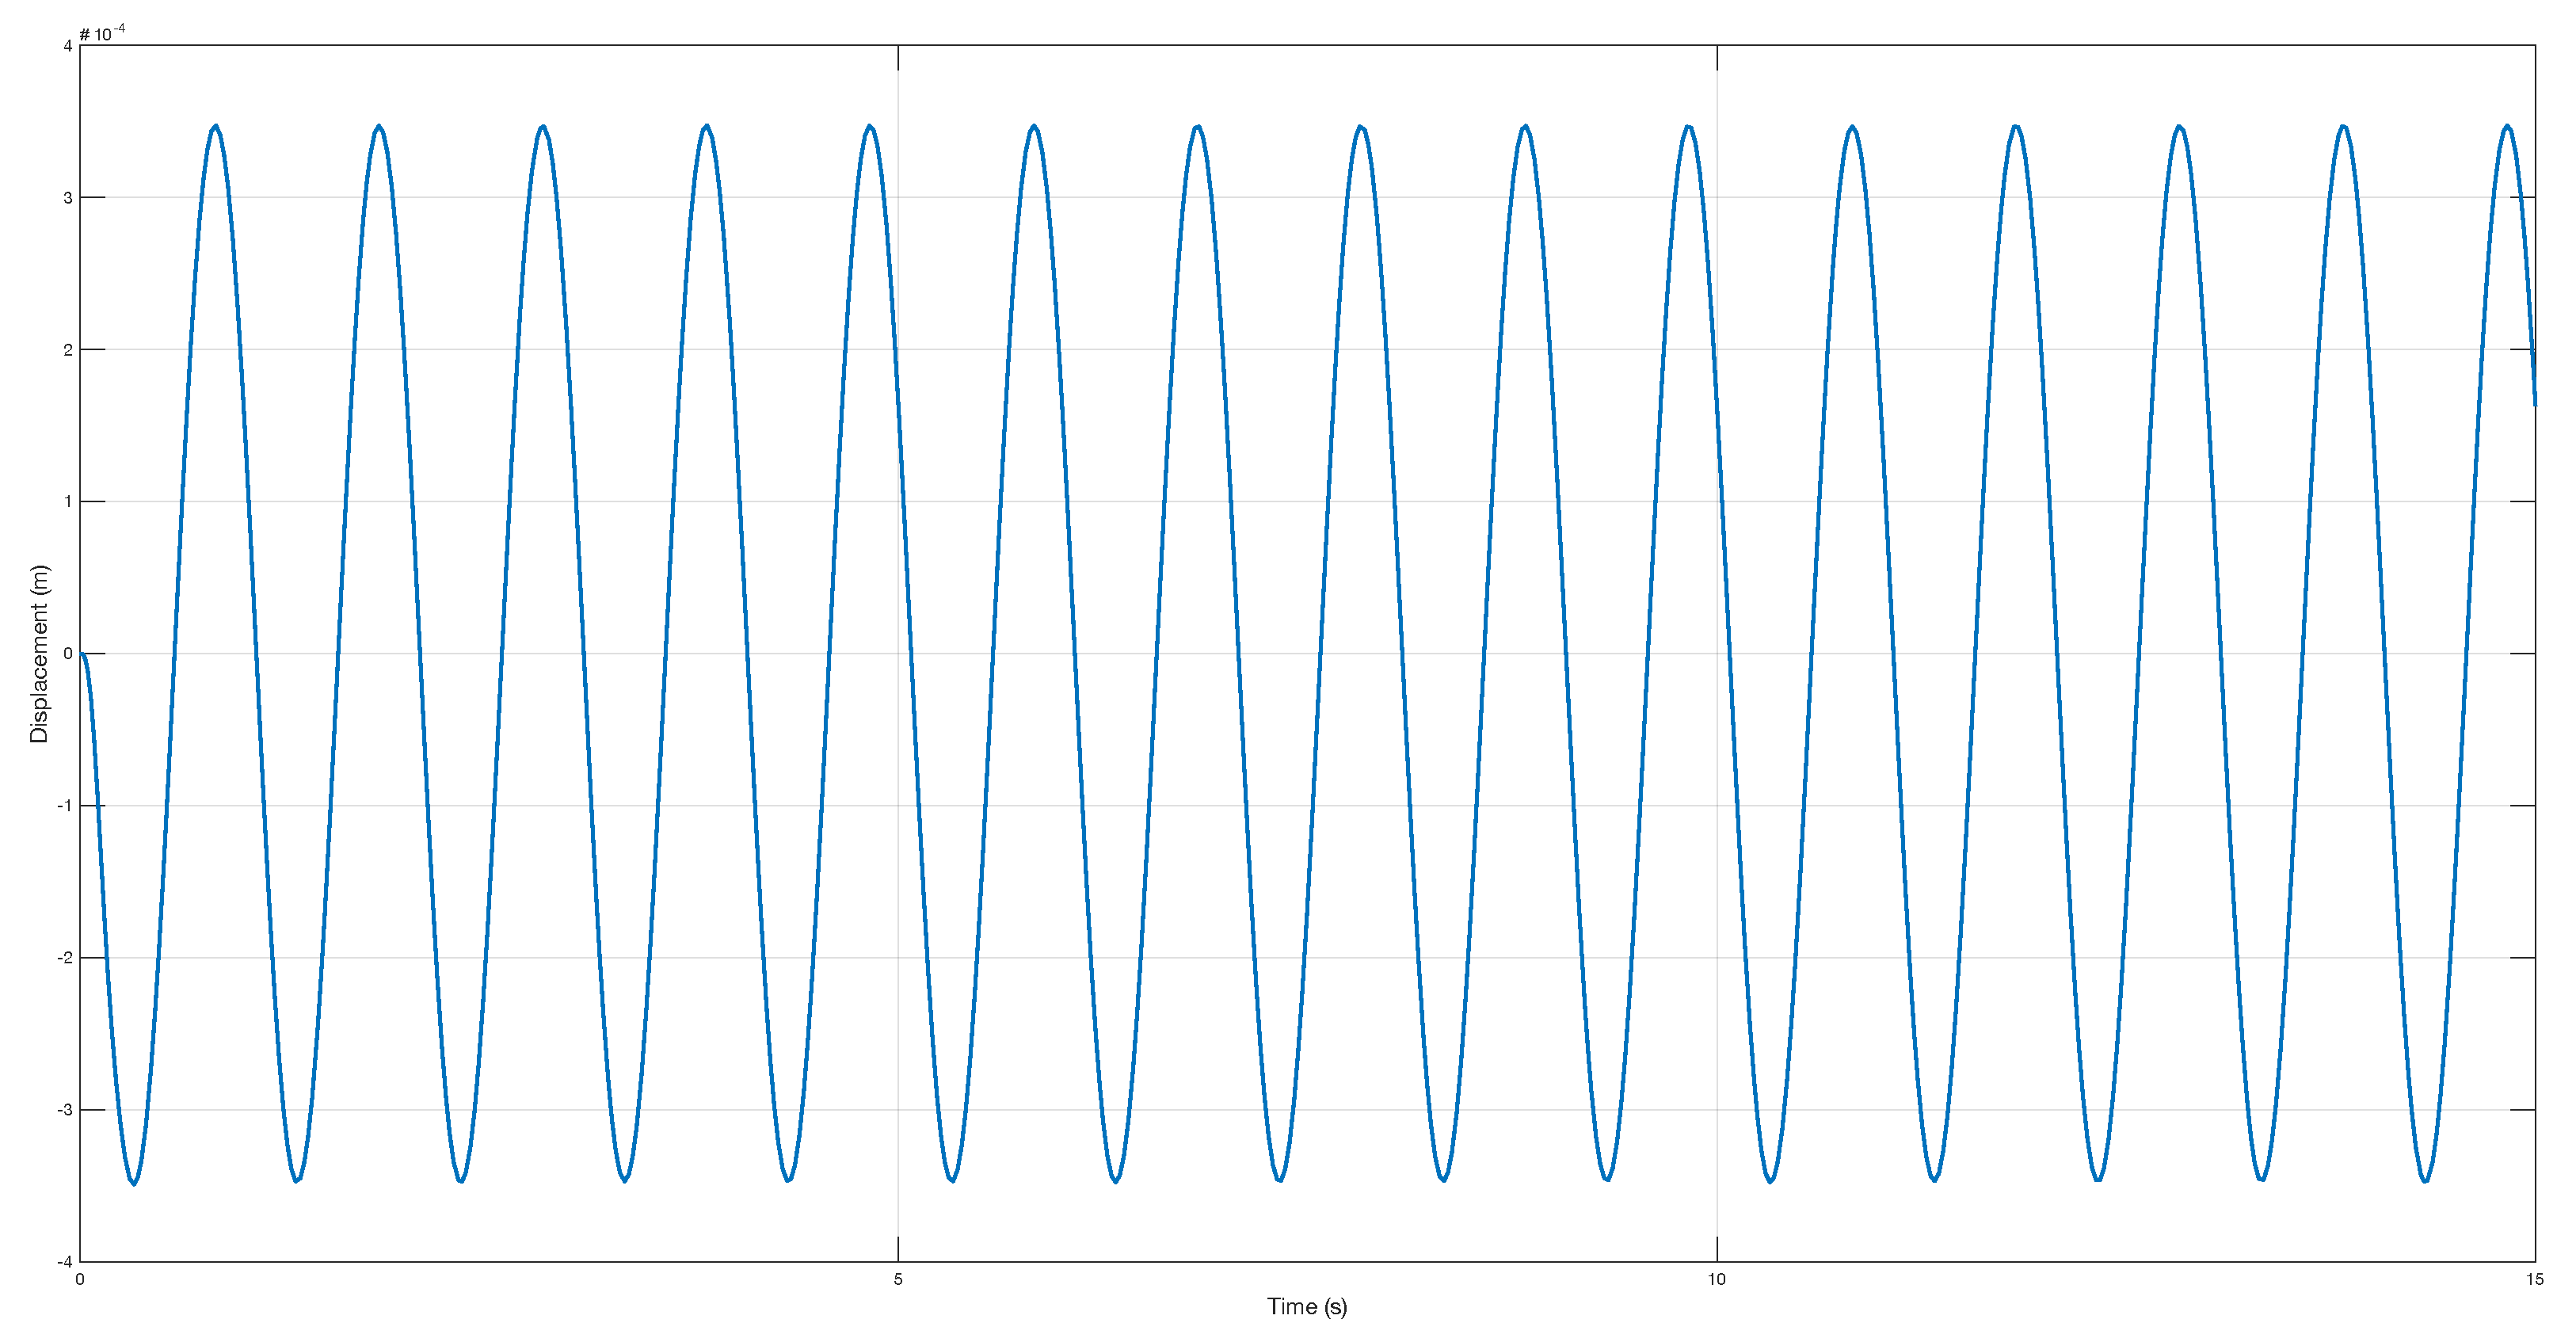
\includegraphics[width=0.8\textwidth]{resources/pdf/output.pdf}
    \caption{Plot of the output of the controlled system}
    \label{fig:output}
\end{figure}

% Gang of four
\subsection{Gang of four}
\subsubsection{Sensitivity function}
$$
S(s) = \dfrac{1}{1 + PC}
$$
The Bode plots of the sensitivity function are given at figure \ref{fig:sensitivity}. That function tells us how the noise acts on the output. We do not want the system to react to the noise, as it is actually the measurement noise that must stay in the output.\par
That noise is a high-frequency phenomenon and, as can be seen on the Bode plots, there is no attenuation for high frequency, which is what we want.
\begin{figure}[H]
    \centering
    \includegraphics[width=0.8\textwidth]{resources/png/sensitivity.png}
    \caption{Bode plots of the sensitivity function}
    \label{fig:sensitivity}
\end{figure}

\subsubsection{Load sensitivity function}
$$
PS(s) = \dfrac{P}{1 + PC}
$$
This function tells us how the disturbances act on the output and the Bode diagrams are given at figure \ref{fig:load}. Our system needs to be robust against disturbances. In our case, these disturbances are low frequency phenomena (frequency of the wind, which we have either chosen constant or a sine function of frequency equal to 1). We can see that we have a very good reaction concerning the effect of the wind on the output of the system (attenuation of more than \SI{-200}{\deci\bel}).
\begin{figure}[H]
    \centering
    \includegraphics[width=0.8\textwidth]{resources/png/load.png}
    \caption{Bode plots of the load sensitivity function}
    \label{fig:load}
\end{figure}

\subsubsection{Complementary sensitivity function}
$$
PS(s) = \dfrac{PC}{1 + PC}
$$
This function tells us how the disturbances act on the controllable input and the reference acts on the output, and the Bode diagrams are given at figure \ref{fig:complementary-sensitivity}.\par
The control signal must be reactive to disturbance and the output should be able to track the reference. Amplitudes at low frequency should therefore not be dampened, and we see that they are not attenuated on the plots.
\begin{figure}[H]
    \centering
    \includegraphics[width=0.8\textwidth]{resources/png/complementary-sensitivity.png}
    \caption{Bode plots of the complementary sensitivity function}
    \label{fig:complementary-sensitivity}
\end{figure}

\subsubsection{Noise sensitivity function}
$$
PS(s) = \dfrac{C}{1 + PC}
$$
This function tells us how the noise and the reference act on the controllable input, and the Bode diagrams are given at figure \ref{fig:noise-sensitivity}.\par
That function should be reactive to reference changes, but not to noise, and so have a high magnitude at low frequency and low magnitude at high frequencies. We can see that it is not the case here. Indeed, we have high amplitudes for high frequencies. However, as our reference does not change in our system (we do not plan on dampening the oscillations in a Pisa Tower), it does not really matter.\par
It is also known that temporal domain controllers are better at reacting to reference changes than frequency domain ones.
\begin{figure}[H]
    \centering
    \includegraphics[width=0.8\textwidth]{resources/png/noise-sensitivity.png}
    \caption{Bode plots of the noise sensitivity function}
    \label{fig:noise-sensitivity}
\end{figure}

% Delays
\subsection{Delays}
We have delays in our system that are due to the sensor transmitting the information, the microcontroller processing that information and the actuator (piston) actually moving our mass damper. We have chosen that last source of delay as being the biggest one, with a frequency of \SI{50}{\hertz}, which induces delays of \SI{0.02}{\second}.\par
Some Bode and Nyquist plots showing delays are given at figures \ref{fig:bode-70}, \ref{fig:nyquist-70} and \ref{fig:nyquist-1}.\par
As can be seen, for a phase margin of \SI{70}{\degree}, the delays in our system do not bring instabilities. However, something strange is that a bigger phase margin seems to make our system less robust to delays, as can be seen on the two Nyquist plots given below. That is not how it should be, theoretically speaking. However, we have compared with the way you have designed your components, and do not see a difference.\par
Our lead compensator and gain have the same \og{}form\fg{} as the ones you have used. We have therefore included the Matlab script we have used to plot these figures in the mail we sent.
\begin{figure}[H]
    \centering
    \includegraphics[width=0.8\textwidth]{resources/png/bode-70.png}
    \caption{Bode plots for various delays and a phase margin of 70 degrees.}
    \label{fig:bode-70}
\end{figure}
\begin{figure}[H]
    \centering
    \includegraphics[width=0.8\textwidth]{resources/png/nyquist-70.png}
    \caption{Nyquist plots for various delays and a phase margin of 70 degrees.}
    \label{fig:nyquist-70}
\end{figure}
\begin{figure}[H]
    \centering
    \includegraphics[width=0.8\textwidth]{resources/png/nyquist-1.png}
    \caption{Nyquist plots for various delays and a phase margin of 1 degree.}
    \label{fig:nyquist-1}
\end{figure}

% Noise
\subsection{Noise}
to do

% Feedforward
\subsection{Feedforward}
to do
